\documentclass{ctexart}
\usepackage{CJK}
\usepackage{ctex}
\usepackage{amsmath}
\usepackage{latexsym}
\usepackage{amssymb}
\usepackage[all]{xy}
\usepackage{pgfplots}
\usepackage{tikz}
\usepackage{eso-pic}
\usepackage{geometry}
\usepackage{soul}
\usepackage{ctex, draftwatermark, everypage}
\usepackage{color, soul}
\SetWatermarkText{DRAFT}
\SetWatermarkLightness{0.95}
\SetWatermarkScale{0.4}
\geometry{a4paper}
\begin{document}
\begin{center}
~\\
\ \Huge{\textit{Notes on Renormalization Group}}\\
\end{center}
~\\
~\\
\begin{center}  % 居中
    \begin{figure}[htpb]
    \begin{center}
       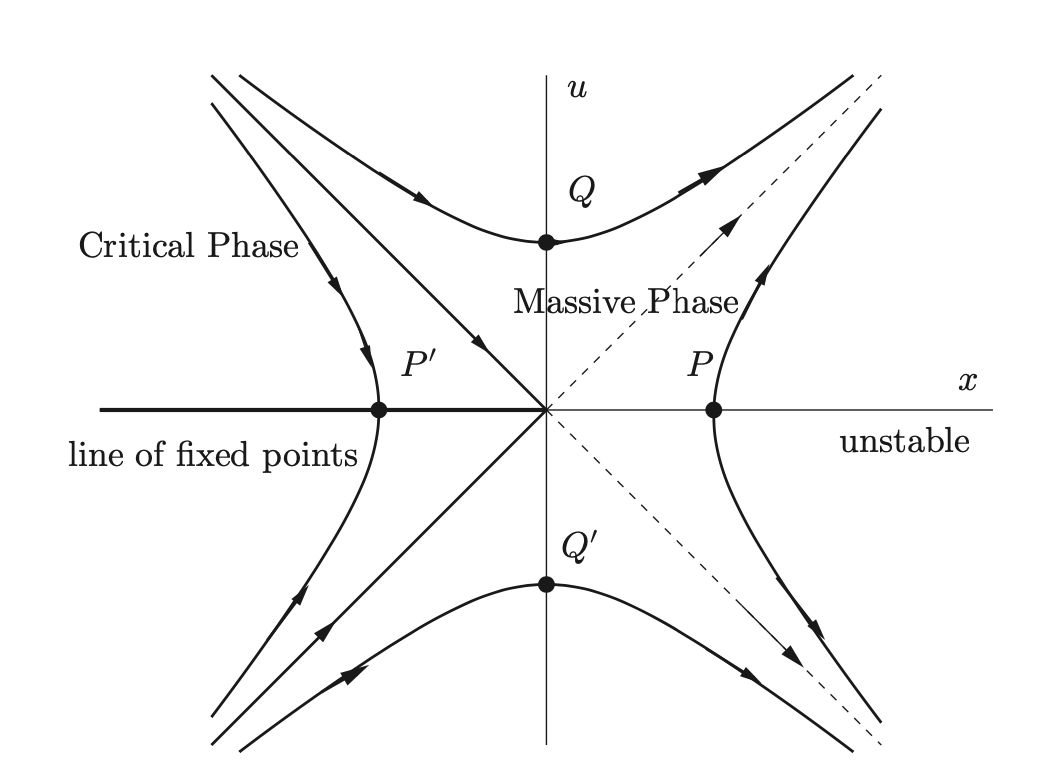
\includegraphics[width=14cm]{截屏2020-08-04 下午5.05.36.png}
    \end{center}
    \end{figure}
\end{center}
\begin{center}
    ~\\
        \huge{\textit{2020.8.1}}\\
    \end{center}\newpage
    \tableofcontents\newpage
\section{标度不变性}
在本章当中将介绍研究有关系统平衡临界行为方法的基本概念“重整化群”.与重整化有所不同的是重整化群可以被用于与场论无关的领域.\par 
凝聚态领域当中的很多问题可以用形如以下的哈密顿量进行刻画$H=H^{*}+H^\prime$,同样的对于作用量也有相同的形式.在经典的统计场论与量子场论当中我们都可以把系统用路径积分表示:
$$\mathcal{Z}=\int \mathcal{D}\phi e^{-S(\phi)}$$
重整化群最简单的表示就是将具有一连串耦合常数和一个标度(代表短程或者高能截断)的系统映射到一个等价的具有另外一些耦合常数和标度的系统.这个过程由所谓的“块-自旋”变换完成.在"自旋-块"变换过程当中,代表短程物理的自由度被积掉,而为了满足单位元不变,随后的标度变换改变了原有的标度.\par 
考虑场$\phi(x,t)$,它由很多傅立叶分量相加而成:
$$\phi(x)=\int\frac{d^Dk}{(2\pi)^D}e^{ikx}\phi(k)$$
那些大动量分量对应着具有更大作用量的位形(记为$\phi_{>}(x)$),如果这些分量被积分积掉了,我们就可以得到$\phi_{<}(x)$对应的有效作用量.在实空间当中我们消除短程的自由度,或者定义在短程标度$ba$(a是晶格常数),波矢$|k|<\frac{\Lambda}{b}$($\Lambda$是高能截断)上的平均位形.\par 
很多情况下$S(\phi)$会在这样的过程当中变化
$$\mathcal{Z}=\int\mathcal{D}\phi_{<}\mathcal{D}\phi_{>}e^{-S(\phi_{<}+\phi_{>})}$$
其中$$\phi=\phi_{<}+\phi_{>}$$
所以$$\mathcal{Z}=\int\mathcal{D}\phi_{<}e^{-S_{eff}(\phi_{<})}$$
如此我们得到了有效作用量
$$e^{-S_{eff}(\phi_{<})}=\int\mathcal{D}\phi_{>}e^{-S(\phi_{<}+\phi_{>})}$$
这就是所谓的“块-自旋”变换.\par 
但是现在我们有一个新的短程截断$a^\prime=ba(b>1)$,或者等价的有高能截断$\Lambda^\prime=\Lambda/b<\Lambda$因此我们需要重新标定长度和时间来还原单位.为了弥补单位元的变化,我们需要重新标定长度和动量:
$$x^\prime=\frac{x}{b}\quad k^\prime=kb$$
使得$|k^\prime|<\Lambda$和$|x|^\prime>a$重新出现.\par 
事实上很多这种变换可以被定义,并且有效作用量的形似依赖于这种定义.但是这种变换必须服从某些最基本的原则.最重要的一条是这个过程必须与物理系统的对称性和睦相处.因此如果系统有各向异性的趋势,则重标度必须与此自洽.简单起见,在接下来的内容当中我们会假设重标度是各向同性的.因此我们假设系统具有有效的洛伦兹对称性.\par 
假设我们能够找到一个作用量$S^*$使得它在重整化群变换下(以下简称RG变换)保持不变.
$$S^*_{eff}(\phi_{<})=S^*(\phi)$$
我们就称这个作用量是RG的固定点(\textit{fixed point})\par 
在固定点作用量和哈密顿量在RG变换下保持不变,处于固定点系统有一个新的对称性:标度不变性(\textit{scale invariance}),因此固定点作用量描述了:
\begin{enumerate}
    \item 关联长度为0的系统,$\xi\rightarrow 0$,因此具有一个发散的能隙,$E_g\rightarrow \infty$,或者
    \item 关联长度无穷的系统,$\xi\rightarrow \infty$,因此无能隙,$E_g\rightarrow 0$.
\end{enumerate}
第一种情况刻画了物质的稳定相$(\textit{stable phase of matter})$.相反的,具有发散关联长度的固定点刻画了物质的临界相$(\textit{systems at criticality})$,因此对应着相变.我们将会看到关联长度为0的固定点在对作用量的微扰下是稳定的,因此称为稳定固定点.相反关联长度发散的固定点是不稳定的,因此称为不稳定固定点.\par 
让我们考虑一个靠近固定点的系统.一般的我们可以将系统的作用量写成
$$S(\phi)=S^*(\phi)+\int dx^D\sum_{n}\lambda_{n}\phi_n(x)$$
其中$\{\phi_n(x)\}$是一组算子,$\{\lambda_n\}$是与之关联的耦合常数.在包括如下步骤的RG变换下:
\begin{enumerate}
    \item 将高能模$\Lambda\rightarrow b\Lambda(b<1)$积掉
    \item 重标度长度$x\rightarrow b^{-1}x$
\end{enumerate}
处于固定点的作用量$S^*(\phi)$保持不变,算子的重标度变换如下:
$$\phi_n(xb^{-1})=b^{\Delta_n}\phi_n(x)$$
$\Delta_n$是算子的标度维数(\textit{scaling dimesion}).在重标度变换下不可约变换的场称为初场$(\textit{primary field})$.因此微扰项变换如下:
$$\int dx^D\sum_{n}\lambda_n\phi_n(x)\longrightarrow \int dx^D\sum_{n}b^{-D+\Delta_n}\lambda_n\phi_n(x)$$
因此RG变换等价于耦合常数的重标度:
$$\lambda^\prime=\lambda_nb^{\Delta_n-D}=\lambda_n(b)$$
既然$b\rightarrow 1^-$,我们可以记作$b=e^{-\delta l}$并且将变换转变成一个耦合常数的可微变换:
$$\beta(\lambda_n)=\frac{\partial\lambda_n}{\partial l}=(D-\Delta_n)\lambda_n+\cdots$$
省略号代表了$\beta$函数的高阶贡献,上述方程通常称为树层$beta$函数(\textit{tree-level beta function})\par 
我们可以定义无量纲耦合常数$\bar{\lambda}_n=\lambda_na^{D-\Delta_n}$.考察在UV截断改变的时候,保持有量纲耦合常数不变的同时我们要如何改变这个无量纲的耦合常数.对于一个无穷小变换$a\rightarrow a+da$可以表述如下:
$$a\frac{\partial\lambda_n}{\partial a}=0\Rightarrow \beta(\bar{\lambda}_n)=a\frac{\partial\bar{\lambda}_n}{\partial a}|_{\lambda_n}=(D-\Delta_n)\bar{\lambda}_n+O(\bar{\lambda}_n^2)$$
从现在开始$\lambda_n$将用于表示无量纲的耦合常数,而我们将会把RG流表示成无量纲耦合常数的变化.物理的原因是由于有量纲的参数取决于单位元的随意选取.\par 
\begin{enumerate}
    \item 如果$D-\Delta>0$,耦合常数$\lambda_n$随着动量标度减小而增减.在这种情况下$\phi_n(x)$是相关算符$(\Delta_n<D)$并且驱动系统远离固定点作用量$S^*$,进入一个新的稳定固定点.
    \item 如果$D-\Delta_n<0$,耦合常数$\lambda_n$随着动量标度减小而减小.在这个情况下$\phi_n(x)$是无关算符$(\Delta_n>D)$,其影响在长程低能下可以被忽略.
    \item 如果$D-\Delta_n=0$,对于头一项而言,耦合常数$\lambda_n$保持不变,在这个情况下$\phi_n(x)$是边缘算符$(\Delta_n=D)$,为了估算它的影响需要进行高阶的计算,如果这个算符确实是微不足道的,则它应该归入固定点作用量当中.
\end{enumerate}
\section{固定点的例子}
固定点作用量的一个最简单的例子就是$D$维的自由标量场.在$D=2$维的情况下是一种最有意思的情况,代表着经典的2维空间统计系统或者$(1+1)$维的量子场论.在下一章我们将会看到这个理论在一维的量子反铁磁系统和Luttinger液体当中扮演着重要的角色.在经典的统计物理当中这是刻画Laudau和Ginzburg发明(最终由Wilson,Fisher和Kadanoff完善)的理论.\par 
D维情况下自由标量场的作用量为
$$S(\phi)=\frac{1}{2}\int d^D x(\partial\phi)^2=\int^\Lambda\frac{d^D k}{(2\pi)^D}\frac{k^2}{2}|\phi(k)|^2$$
其中$\Lambda$是大动量截断.\par 
让我们现在将场分解成快场和慢场两个分量
$$\phi(x)=\phi_<(x)+\phi_{>}(x)$$
其中
$$\phi_{<}(x)=\int^{b\Lambda}\frac{d^D k}{(2\pi)^D}\phi(k)e^{ikx}$$
代表着慢场,而
$$\phi_{>}(x)=\int_{b\Lambda}^{\Lambda}\frac{d^D k}{(2\pi)^D}\phi(k)e^{ikx}$$
代表着快场.在快场和慢场的傅立叶变换下作用量有以下形式
\begin{align*}
    S_{\Lambda} & =S_{<}+S_{>}\\
    & = \int^{b\Lambda}\frac{d^D k}{(2\pi )^D}\frac{k^2}{2}|\phi_{<}(k)|^2+\int^{\Lambda}_{b\Lambda}\frac{d^D k}{(2\pi)^D}\frac{k^2}{2}|\phi_{>}(k)|^2
\end{align*}
其中我们已经将作用量标记上了截断$\Lambda$.因此,当且仅当对于一个自由的场,总的作用量是快场模和慢场模对应的作用量独立之和.在这种简单的情况下我们可以把快场积分积掉从而得到慢场的有效作用量:
$$\int \mathcal{D}\phi_>e^{-S_{\Lambda
}(\phi)}=constant\times e^{-S_{b\Lambda}(\phi_{<})}$$
我们现在必须做一个标度变换从而将截断$b\Lambda$切换到它原来的量:
$$x^\prime=xb^{-1}\quad k^\prime=bk\quad \phi(x^\prime)=b^\Delta\phi(x)$$
在这样的标度变换下场量变换了$b^\Delta$倍,$\Delta$是场的标度维数(\textit{scaling dimesion}),所以在标度变换下
$$\int d^D x\frac{1}{2}\left(\frac{\partial\phi}{\partial x}\right)^2=\int d^D x^\prime b^{2-D}\frac{1}{2}\left(\frac{\partial(x^\prime b^{-1})}{\partial x^\prime}\right)^2$$
因此如果标度维数等于$\Delta=\frac{D-2}{2}$的话那么作用量在标度变换下就是不变的.$D=2,\Delta=0$的情况是特殊的.\par 
我们现在考虑对固定点的微扰.质量项$\int d^D(\frac{m^2}{2})\phi^2$在重标度变换下并不是不变的,因为体积项变化为$\int d^2 x\rightarrow d^D x^\prime b^{-D}$以及$\phi^2\rightarrow b^{2\Delta}\phi^2$,所以质量项要按$m^{\prime2}=b^{2\Delta-D}=b^{-2}m^2$进行变换,所以随着$b$的变小耦合常数$m^2$在重整化下流向更大的值.\par 
与此相似的,高阶导数算符的耦合常数随着$b$的变小而变小,
$$\int d^D xg(\partial^2\phi)^2=\int d^D x^\prime b^2g(\partial^{\prime2}\phi^\prime)^2$$
因此$g^\prime=gb^2$,我们得到了在RG变换下$g$随着$b$一起变小,这是一个无关算符.显然的,更高阶导数的算符将会更加无关.这与有效场理论在长程内必须只包含与对称性相容的最小的可能导数项算符的直觉是自洽的.\par 
同样的结论从简单的量纲分析当中也可以得到.通过要求自由场作用量应该是无量纲的,我们发现标量场的单位是$[\phi]=L^{-\Delta}$,其中$\Delta=\frac{D-2}{2}$是标度维数.类似的,质量的单位是$L^{-1}$.同样的原因也决定了相互作用项的标度.通过重新要求这些项是无量纲的,我们发现$L^D[\lambda_r][\phi]^r=1$,因此$\phi^r$的标度维数是$\Delta_r=r\Delta=r\frac{D-2}{2}$.因此耦合常数的单位就是$[\lambda_r]=L^{-D+\Delta}$.比如说$[\lambda_4]=L^{D-4}$,则其在$D=4$的情况下是无量纲的.对于无量纲的耦合常数$\lambda_r$我们同时也可以写下树层$\beta$函数
$$\beta(\lambda_r)=(D-\Delta_r)\lambda_r+O(\lambda_r^2)$$
所以对于无质量自由标量场,其固定点是稳定的如果$D-\Delta_r<0$,但是因为
$$D-\Delta_r=\frac{r-2}{2}\left(-D+\frac{2r}{r-2}\right)$$
只有在$D>\frac{2r}{r-2}$的情况下固定点才是稳定的.特别的,算符$\phi^4$是无关的当且仅当$D>4$并且对于$D<4$自由场的固定点是不稳定的.
\subsection{非线性$\sigma$模型}
在第七章当中我们会介绍作为量子反铁磁系统的场论——非线性$\sigma$模型,例如对于一个$N$分量的标量场,满足约束$\vec{n}^2=1$.由于这个约束使其不再是一个自由场.同时约束要求场$\vec{n}$是没有量纲的.非线性$\sigma$模型的作用量是:
$$S=\frac{1}{2g}\int d^D x(\partial_\mu \vec{n})^2$$
对于$\mu=1,\cdots, D$. 作用量当中的唯一算符有着$\Delta=2$的标度维数.考虑到对称性的原因,只有导数算符才被允许出现,并且具有更高阶导数的算符会对应着具有一个更大的标度维数.根据量纲分析我们发现耦合常数的单位为$[g]=L^{D-2}$,因此在$D=2$的情况下它是无量纲的.耦合常数$g$的树层$\beta$函数是$\beta(g)=-(D-2)g+\cdots$.因此量纲分析预言在$g\rightarrow 0$处出现固定点,对于$D>2$在经典理论当中刻画了一个稳定相.我们会在第七章当中更多的讨论这个问题.\par 
\subsection{费米液体当中的标度}
费米液体是有限密度的费米子系统,在许多情况下,由于费米表面的存在所施加的运动学约束,它们的相互作用在低能量下变得非常弱,一维情况除外.在这个极限下,相互作用的系统平滑地与非相互作用的费米准粒子的物理联系起来。这反映在这些系统表现出的简单缩放行为上,这是费米液体的朗道理论的本质.\par 
无相互作用费米子系统是用由单粒子谱为$\epsilon(p)$的费米子场构成的作用量来描述的.费米面是一个由$\epsilon(p)=E_F$构成的$\{p\}$轨迹.在足够低能的情况下,例如靠近费米能级,费米态所允许的能量被约束在费米面附近并且这些激发态的能量稍微偏离$E_F$.在这个形式下将单粒子谱做近似$\epsilon(p)=v_F(|\vec{p}|-p_F)+\cdots$是合理的.其中$v_F$是费米速度,$p_F$是费米动量.因此在这个极限下动量和能量表现出相同的标度行为,所以时间和空间也表现出相同的标度行为. (Polchinski, 1993; Shankar, 1994),$T\sim L$,所以动力学临界指数为$z=1$. 但是考虑到只有动量的切向分量表现出标度行为,切向分量并不改变能量,这种情况下准粒子之间的相互作用事实上表现为无关(除了Cooper channel).这种相互作用的普遍的无关性是Landau费米液体理论鲁棒性的原因.
\subsection{自由相对论费米子理论}
自由相对论费米的系统服从Dirac方程.在凝聚态物理当中相互作用狄拉克费米子自然出现在一维的费米子系统当中比如说Luttinger液体.它们也出现在一维反铁磁系统当中的拓扑激发(或者孤子).狄拉克费米子为石墨烯当中的低能电子态提供来自然的描述,以及d波超导当中的费米准粒子.\par 
狄拉克费米子是旋量场.狄拉克费米子在一维或者两维的空间当中是4分量场.假设$\Psi_\alpha,\alpha=1,2$,代表着空间维数为$D=1+1,D=1+2$的2分量费米场.在$D=1+1$的维数当中,两分量代表着左右移动的费米子.$D=1+1$当中的无质量狄拉克费米子的哈密顿密度是
$$\mathcal{H}=v_F\Psi_{\alpha}^\dagger i\sigma_3^{\alpha\beta}\partial_x\Psi_{\beta}(x)$$
单粒子谱的形式为$E(p)=v_Fp$.在无能隙(质量为0)的极限下,单粒子谱是线性的.因此时间和空间的标度行为是相同的$T\sim L$,相对论不变性要求狄拉克费米子的动力学临界指数为$z=1$.\par 
自由狄拉克场的作用量为
$$S=\int d^2 x\bar{\Psi}_\alpha(x)i\gamma_{\alpha\beta}^{\mu}\partial_\mu\Psi_\beta(x)$$
其中我们用到了狄拉克$\gamma$矩阵,$\gamma_0=\sigma_1,\gamma_1=-i\sigma_2$以及$\bar{\Psi}=\Psi^{\dagger}\gamma^0$
在这个相对论性的记号下费米速度$v_F$通过重新定义时间$x_0=v_F t$被吸收进时间项当中.(与光速类似)\par 
自由狄拉克费米子是标度不变的.可以直接去求出在固定点处不同局域算符的标度行为.通过将上式的作用量推广到$D$维时空,仙子我们有$D$个反对易的\textit{gamma}矩阵$\gamma_\mu$.我们看到狄拉克场的标度为$[\Psi]=L^{-(D-1)/2}$。很容易求出一些简单局域算符的标度,比如说质量项$\bar{\Psi}\Psi$的临界维数为$\Delta=D-1$,因此狄拉克质量$[m]=L^{-1}$.标度分析显示狄拉克流$j_\mu=\bar{\Psi}\gamma_\mu\Psi$的标度维数为$D-1$.\par 狄拉克费米子的局域相互作用为四费米子算符,比如说$\bar{\Psi\gamma_\mu\Psi}^2$和$(\bar{\Psi}\Psi)^2$,其标度维数为$\Delta=2(D-1)$,特别的在$D=1+1$当中,流的维数为1,四费米算符维数为2.因此在2维空间当中四费米算符的是边缘的,在$D>2$的情况下是无关的.与之相关联的耦合常数$g$为$[g]=L^{D-2}$.因此树图$\beta$函数为
$$\beta(g)=-(D-2)g+O(g^2)$$
这与非线性$\sigma$模型是类似的.\par 
因此无质量狄拉克费米子理论是重整化群的一个固定点.其中在$D=1+1$的情况下固定点是边缘稳定的.就像在非线性西格玛模型的情况下,我们将看到,确定这个不动点的实际稳定性需要我们考虑在$\beta$函数$O(g^2)$阶出现的波动的影响.从另外一方面看来,$D>2$的无质量狄拉克费米子固定点在小的局域微扰下是稳定的,定义了一个稳定相.因此对于$D>2$的具有四费米相互作用的相对性费米子理论是微扰稳定的(红外情况下),并且在耦合常数到达临界值的时候相移到一个有能隙到相当中.石墨烯就是一个例子。当$D < 4$时,自由狄拉克不动点相对于与动态规范场的耦合是不稳定的。控制这一理论的红外行为的不动点的性质还没有被很好地理解.\par 
\section{可观测量的标度行为}
重整化群的一个强有力的应用就是假设已经了解了固定点,我们就能知道物理体系当中的可观测量的行为.这也是经典理论和量子理论当中临界现象理论的基础.
\subsection{关联长度}
我们将从开始研究系统在固定点附近的关联长度$\xi$的行为.距离固定点的距离是由无量纲耦合常数$\lambda$所控制的.根据量纲分析我们可以将$\xi$写成以下的形式:
$$\xi=af(\lambda)$$
其中$f(\lambda)$是一个目前为止还没有确定的耦合常数的无量纲函数,$a$是耦合常数.\par 
根据物理有量纲量的要求,系统的关联长度在重整化群变换下是不变的,我们可以得到所谓的确定$f(\lambda)$流方程(\textit{flow equation}).所以根据条件
$$\frac{\partial{\xi}}{\partial lna}=0=\frac{\partial}{\partial ln a}(af(\lambda))$$
可以得到$f(\lambda)$的微分流方程
$$0=af(\lambda)+a\frac{f}{\partial\lambda}\frac{\partial\lambda}{\partial lna}$$
其中我们定义上式右边的最后一项$(Gell-Mann-Low)\beta$函数,$\beta(\lambda)=a\frac{\partial \lambda}{\partial a}$
我们现在可以将流方程写成
$$0=f(\lambda)+\frac{\partial f}{\partial \lambda}\beta(\lambda)$$
这种形式的流方程被称为Callan-Symanzik,或者重整化群方程.\par 
如果$\beta$函数已经知道了,解这些流方程是很平庸的,它们是一阶微分方程,最简单的情况下我们可以得到
$$\frac{\partial ln f}{\partial \lambda}=-\frac{1}{\beta(\lambda)}$$
这说明$f(\lambda)$的形式必须为
$$lnf(\lambda)=constant-\int\frac{d\lambda^\prime}{\beta(\lambda^\prime)}$$
两边做积分我们得到最后的解
$$ln\left(\frac{f(\lambda)}{f(\lambda_0)}\right)=-\int_{\lambda_0}^{\lambda}\frac{d\lambda^\prime}{\beta(\lambda^\prime)}$$
我们现在考虑的理论在固定点的时候无量纲耦合常数有一个特别的值$\lambda^*$.固定点被定义在$\beta$函数为0的点$\beta(\lambda^*)=0$.\par 
让我们考虑系统处于两个无量纲耦合常数$\lambda_1,\lambda_2$的情况,关联长度的取值为$\xi(\lambda_1)=af(\lambda_1),\xi(\lambda_2)=af(\lambda_2)$,则$f(\lambda_1),f(\lambda_2)$有着以下的形式
$$f(\lambda_1)=f(\tilde{\lambda})exp\left(\int_{\lambda_1}^{\tilde{\lambda}}\frac{d\lambda}{\beta(\lambda)}\right)$$
和
$$f(\lambda_2)=f(\tilde{\lambda})exp\left(\int_{\lambda_2}^{\tilde{\lambda}}\frac{d\lambda}{\beta(\lambda)}\right)$$
其中$\tilde{\lambda}$是耦合常数的某个值,因此关联长度的比例为$$\frac{\xi(\lambda_1)}{\xi(\lambda_2)}=exp\left(\int_{\lambda_1}^{\tilde{\lambda}}\frac{d\lambda}{\beta(\lambda)}-\int_{\lambda_2}^{\tilde{\lambda}}\frac{d\lambda}{\beta(\lambda)}\right)=exp\left(\int_{\lambda_1}^{\lambda_2}\frac{d\lambda}{\beta(\lambda)}\right)$$
因此我们发现了$$\xi(\lambda_1)=\xi(\lambda_2)exp\left(\int_{\lambda_1}^{\lambda_2}\frac{d\lambda}{\beta(\lambda)}\right)$$
在固定点$\lambda^*$附近可以做如下近似
$$\beta(\lambda)=\beta^\prime(\lambda^*)(\lambda-\lambda^*)+O((\lambda-\lambda^*)^2)$$
其中$\beta^\prime(\lambda^*)$是$\beta$函数在固定点的梯度.如果我们取$|\lambda_1-\lambda^*|<<\lambda^*$非常接近固定点,以及$|\lambda_2-\lambda^*|\approx\lambda^*$离固定有着一段有限的距离,则方程变为
\begin{align*}
    \xi(\lambda_1) & =\xi(\lambda_2)exp\left(\int_{\lambda_1}^{\lambda_2}\frac{d\lambda}{\beta^\prime(\lambda^*)(\lambda-\lambda^*)+\cdots}\right)\\
    & =\xi(\lambda_2)exp\left[\frac{1}{\beta (\lambda^*)}ln\left(\frac{\lambda_2-\lambda^*}{\lambda_1-\lambda^*}+\cdots+\right)\right]\\
    & =\xi(\lambda_2)\left(\frac{\lambda_2-\lambda^*}{\lambda_1-\lambda^*}\right)^{1/\beta^\prime(\lambda^*)}
\end{align*}
如果耦合常数$\lambda$对应的算符是关联算符的化,则$\beta$函数的梯度一定要是正的,$\beta^\prime(\lambda^*)>0$.在这种情况下,假设关联算符驱动系统到一个具有有限关联长度 $\xi(\lambda_2)\approx a$的相,上述的方程暗示了在靠近固定点$\lambda\rightarrow \lambda^*$的时候,关联长度$\xi(\lambda)$必须按某种幂律发散,
$$\xi(\lambda)\approx a
\left|\frac{\lambda_2-\lambda^*}{\lambda-\lambda^*}\right|^{\nu}$$
其中$$\nu=\frac{1}{\beta^\prime(\lambda^*)}$$
是普适临界指数(\textit{universal critical exponent}).一般的我们发现$\nu$是独立于系统的微观物理的,并且也独立于短程截断$a$的选择.总之在靠近固定点$\lambda\rightarrow\lambda^*$时关联长度必须发散,$\xi(\lambda)\rightarrow\infty$,其幂指数为普适临界指数.\par 
\subsection{标度不变性的普遍重要性}
我们现在将讨论固定点处理论的一些基本并且重要的性质.我们注意到在固定点处系统表现出标度不变性,即一种在固定点处精确保持的对称性.我们同时假设系统是均匀各向同性的.紧接着我们会假设在固定点处系统但是关联长度是无穷的,即$\lim_{\lambda\rightarrow \lambda^*}\xi(\lambda)=\infty$并且远远大雨短程截断$a$(晶格间距).在这个体系下等价于将晶格系统重新放置在去离散化的有效场论当中.在量子场论当中,一个具有这种性质的系统可以由共形场论($\textit{conformal theory}$)进行刻画.\par 
在讨论当中我们会采用一个具有启发性的方法并且我们将不会为众多重要有效的性质提供正式的证明.许多证明可以在文献当中获得,例如Polyakov (1987) 和 Cardy (1996).但是为了展示方法的普适性我们将会需要这些性质.\par 
假设$\{\phi_n(\vec{r})\}$是标度不变作用量为$S^*$的系统在固定点处的算子的集合.这里$n$是一串依赖于系统的指标.我们将会假设在标度变换下算符按照$\phi_n(b\vec{r})=b^{-\Delta_n}\phi_n(\vec{r})$.在标度变化下不可约变换的算符称为初算子(或者初场).算子的变换性质支配着关联函数的变换性质.因此作用量的标度不变形要求在全局的标度变换下$\vec{r}\rightarrow\vec{r}$所有的关联函数将会做简单的变换.这意味着固定点处的期望值必须是齐次的.函数是$k$次齐次的,则其在标度变换$x\rightarrow bx$下,其变换类似$F(bx)=b^kF(x)$.\par 
\subsection{标度不变性与关联函数}
我们现在将这个概念应用到固定点$S^*$处算子$\phi_n(x)$的关联函数当中去.下面我们用$\langle\cdots\rangle_*$来标记期望值.我们会假设算符是在固定点处是正规编积的,$\langle\phi_n(\vec{r})\rangle_*=0$
\subsection{固定点处的微扰重整化群}
我们现在可以看到算符的标度维数和OPE的结构常数完全确定了重整化群的$\beta$函数(在固定点的附近),假设在固定点的附近系统的作用量由$S^*$描述:
$$S=S^*+\delta S=S^*+\int d^D x\sum_{n}g_na^{Delta_n-D}\varphi_n(x)$$
$g_n$是无量纲的耦合常数,$a=\Lambda^{-1}$是短程截断,我们假设微扰算符是初场并且满足我们之前所罗列的性质.\par 
现在我们要来考虑$\delta S$所带来的微扰效应.\par 
考虑系统的配分函数
$$Z=tr e^{-S(\varphi)}=tr\left[e^{-S^*}e^{-\sum\int d^D x g_na^{\Delta_n-D}\varphi_n(x)}\right]$$
展开得到
\begin{align*}
    \frac{Z}{Z^*} & =1+\sum\int \frac{d^Dx}{a^{D-\Delta_n}}g_n\langle\varphi_n(x)\rangle^*\\
& +\frac{1}{2!}\sum_{n,m}\int \frac{d^Dx_1}{a^{D-\Delta_n}}\frac{d^Dx_2}{a^{D-\Delta_n}}g_ng_m\langle\varphi_n(x_1)\varphi_m(x_2)\rangle^*\\
& -\frac{1}{3!}\sum_{n,m,k}\int \frac{d^Dx_1}{a^{D-\Delta_n}}\frac{d^Dx_2}{a^{D-\Delta_n}}\frac{d^Dx_1}{a^{D-\Delta_k}}g_ng_mg_k\langle\varphi_n(x_1)\varphi_m(x_2)\varphi_k(x_2)\rangle^*+\cdots
\end{align*}
固定点的关联算符要求具有良好的形式,因此上式的积分出现奇异的现象.有两种具体的形式:
\begin{enumerate}
    \item 长程,红外发散(IR),被一个有限长度$L$(系统长度)所截断.
    \item 短程,紫外发散(UV),被一个短程截断$a$所调整.
\end{enumerate}
在这种形式下,展开看上去像位于$\{x_k\}$某种气体或是粒子的配分函数,其中$n$标记着不同粒子的种类.我们所研究的体系将会是各个粒子距离甚远但是与系统相比仍然微不足道,即
$L>>|x_1-x_2|>>a$.\par 
一个$RG$变换包含
\begin{enumerate}
\item 短程截断的变换$a\rightarrow ba,b=e^{\delta l}>1$. 同过改变耦合常数以确保配分函数不变. 
    首先先观察一下截断变换所出现的位置:积分的$L$依赖性.
    \begin{enumerate}
        \item 作用量当中的$a^{D-\Delta_n}$
        \item 积分当中的截断$a$
        \item 积分的L依赖性
    \end{enumerate}
\item 截断$a$的改变引起的影响已经通过重新标度$g_n$得到解决.事实上在变换$a\rightarrow ba$下耦合常数的变换为
    $$\frac{g_n}{a^{D-\Delta_n}}\rightarrow \frac{g_n}{a^{D-\Delta_n}b^{D-\Delta_n}}$$
    也即
    $$g_n\rightarrow b^{D-\Delta_n}g_n=g_n(1+(\delta l)(D-\Delta_n)+\cdots$$
    因此
    $$g_n\rightarrow g_n+(D-\Delta_n)g_n\delta l+\cdots$$
    由标度维数和维数所决定.容易看到这样的变换等价于$\beta$函数的树图近似.\par 
\item 接下来看看积分当中$UV$截断改变的影响. 截断在这个积分当中体现为约束两个坐标之间的距离$|x_j-x_k|>a$,因此在截断发生改变的时候
$$\int_{|x_j-x_k|>a(1+\delta l)}d^Dx_j d^Dx_k F(x_j,x_k)=\int_{|x_j,x_k|-a(1+\delta l)>|x_j-x_k|>a}d^Dx_jd^D x_kF(x_j,x_k)$$
$a(1+\delta l)>|x_j-x_k|>a$代表着紫外截断变化所带来的影响.\par 
可以看到0阶项和一阶项没有奇点,在二阶项处我们直接对两个算符做OPE得到
\begin{align*}
   \frac{1}{2!} & \sum_{n,m}\int \frac{d^Dx_1}{a^{D-\Delta_n}}\frac{d^Dx_2}{a^{D-\Delta_n}}g_ng_m\langle\varphi_n(x_1)\varphi_m(x_2)\rangle^*\\
   & \equiv \frac{1}{2}\sum_{n,m,k}\int d^Dx_1d^Dx_2\frac{g_ng_m}{a^{2D-\Delta_n-\Delta_m}}\frac{C_{nmk}\langle\varphi_k(\frac{(x_1+x_2)}{2})\rangle^*}{(|x_1-x_2|^{\Delta_n+\Delta_m-\Delta_k})}+\cdots\\
   & =\sum_{nmk}C_{nmk}a^{\Delta_k-\Delta_n-\Delta_m}g_ng_m\int d^Dx\langle\varphi_k(x)\rangle^*\frac{S_Da_D\delta l}{a^{2D-\Delta_n-\Delta_m}}+\cdots\\
   & \equiv \frac{1}{2}\sum_{nm}\sum_{k} g_{n}g_{m}C_{nmk}\int\frac{d^Dx}{a^{D-\Delta_k}}\langle\varphi_k(x)\rangle^*S_D\delta l
\end{align*}
所以
$$g_k\rightarrow g_k-\frac{1}{2}S_D\sum_{n,m}g_ng_mC_{nmk}\delta l+\cdots$$
树图$\beta$函数的一圈修正为
$$\frac{dg_k}{dl}=(D-\Delta_k)g_k-\frac{1}{2}S_D\sum_{nm}C_{nmk}g_ng_m+\cdots$$
重新定义吸收因子,得到一圈$\beta$函数:
$$\beta(g_k)=\frac{dg_k}{dl}=(D-\Delta_k)g_k-\sum_{nm}C_{nmk}g_ng_m$$
所有的微扰重整化群的一圈$\beta$函数都有这个结构.
\end{enumerate}
\section{相关的计算}
\subsection{混合费米子和波色子的重整化群$(arXiv:0906.0014)$}
\subsubsection{费米子的标度:Shankar的RG}
对于费米子,作用量的二次项由以下给出
$$S_2^f=\int d^dKd\epsilon \bar{\psi}(i\epsilon-\xi_{K})\psi$$
为了定义一个标度体系\textit{scaling scheme}保持$\mathcal{S}_2^f$不变,我们复习费米子重整化群的内容.与波色体系不同,低能的费米子处于一个费米球内.
对于费米子来说高能截 断体现为\underline{怎么理解这里的积分范围}
$$\int^\Lambda d^dK=\int \Omega\int_{k_F-\Lambda}^{k_F+\Lambda}k^{d-1}dk,k_F>>\Lambda$$
我们通过假设费米体积不变来设计标度体系.
原体积$\int^{\Lambda/s}d^d K=\Omega_K\int_{k_F-\Lambda}^{k_F+\Lambda}k^{d-1}dk$
很显然没有什么重标度能使得这个积分重新回到原积分的形式.费米子和波色子RG之间差异悬殊.先假设$k=|\vec{k}|-k_F$,$k=0$的时候对应着总能量为0($\xi_k=\frac{k^2-k_F^2}{2m}\approx v_F(k-k_F)=v_F k$)在这个变换下
\begin{align*}
    & \Omega_k\int_{-\Lambda/s}^{\Lambda/s}(k_F+k)^{d-1}dk\\
    & =k_F^{d-1}\Omega_k\int_{-\Lambda/s}^{\Lambda/s}(1+\frac{k}{k_F})^{d-1}dk\\
    & \approx k_F^{d-1}\Omega\int_{-\Lambda/s}^{\Lambda/s}dk
\end{align*}
对$k$做变换$k^\prime=sk$就可以将作用量变回到原来的形式.
\subsection{KT重整化群}
\section{相关结论}
\subsection{Finite-time Scaling and its Applications
to Continuous Phase Transitions
}
\textbf{模型}\par 考虑这样一个模型
\begin{enumerate}
\item Ginzburg-Landau作用量:$S[\varphi]=\int dr\{\frac{1}{2}\tau\varphi^2+\frac{1}{4!}g\varphi^4+\frac{1}{2}(\nabla\varphi)^2-H\varphi\}$
\item 场的运动方程由Langevin方程给出:
$$\frac{\partial\varphi}{\partial t}=-\lambda\frac{\delta F[\varphi]}{\delta\varphi}+\xi$$
\item $\xi$为Gaussian噪声
\item 临界点附近,磁场与温度是随时间线性缓变的.这也导致二次项系数随时间线性缓变.
\end{enumerate}
\underline{通过运用flat unity,做变量替换,可以将Ising模型用低能情况下的$\varphi^4$模型进行描述,}\newline 
\underline{类比的, 这个模型与“kinetic Ising model with local spin dynamics”是同一等价类}\newline\underline{(Hohenberg \& Halperin, 1977).}\par 
\textbf{场论构造}\par 
从Langevin方程得到
$$\dot{\varphi}+\lambda \varphi+\frac{1}{3!}\lambda g\varphi^3-\lambda H+\xi=0$$
引进有效作用量,得到生成泛函
$$\int\mathcal{D}(\varphi,\tilde{\varphi})exp[-I[\varphi,\tilde{\varphi}]+\int drdt(h\varphi+\tilde{h}\tilde{\varphi})]]$$
其中
$$I[\varphi,\tilde{\varphi}]=\int drdt\left\{ \tilde{\varphi}[\dot{\varphi}+\lambda(\tau-\nabla^2) \varphi+\frac{1}{3!}\lambda g\varphi^3-\lambda H]-\lambda\tilde{\varphi}^2\right\}$$
\underline{这个有效作用量的构造方法还是第一次见.}
定量对比一下这个$\varphi4$理论与一般的$\varphi^4$,可以看到这个理论在$t\rightarrow \infty$系数发散,需要引入新的contour term,即出现了新的发散.
\underline{$(\omega\rightarrow 0)$}
\underline{我将其命名为红外频率区.}\par
\textit{(Amit \& Martin-Mayor, 2005; Janssen,1992; Zinn-Justin, 1996)}对这个模型做了一般流程的维数正规化. \underline{这个维数正规化的过程和一般的$\varphi4$理论几乎完全相同,只是多了两个}\newline
\underline{耦合常数$\lambda, H$, 这个理论当中的$\tau$相当于是$m$}. 
\par 
我们把$t=0$时刻设置为$\tau=0,H=0.$
将序参量用生成泛函表示并且对$\tilde{h},\tau$做Taylor展开
$$M(\tau, M)=\langle\varphi\rangle=\sum_{N,N^\prime}\frac{1}{N!N^\prime !}\lambda^{N+N^\prime}\tau^{N^\prime}H^N\frac{\delta^{1+N+N^\prime }W}{\delta h\delta\tilde{h}^N\delta\tau^{N^\prime}}$$
得到RG方程
$$\left(\mu\partial_\mu+\varsigma\lambda\partial_{\lambda}+\beta\partial_u+\gamma_{\varphi^2}\tau\partial_{\tau}+\frac{1}{2}\gamma H\partial_H+\frac{1}{2}\gamma\right)M=0$$
$\xi(u),\gamma(u),\gamma_{\varphi^2},\beta$分别是不同参数的$\beta$函数.
在稳定点处分析$\beta(u^*)=0$,得到
$$M(\lambda,\tau, H,u,\mu)=\rho^{\gamma/2}M(\lambda\rho^\varsigma,\tau\rho^{\gamma_{\varphi^2}},H\rho^{\gamma/2},u,\mu\rho)$$
做量纲分析
最后得到
$$M(t,\tau,H)=b^{-\beta/\nu}M(tb^{-z},\tau b^{1/\nu},Hb^{\beta\delta/\nu})$$
先停下我们的分析,将这个结果与前人得到的结果进行对比
$$M(\tau,H,t,L^{-1})=b^{-\beta/\nu}M(\tau b^{1/\nu},Hb^{\beta\delta/\nu},tb^{-z},L^{-1}b)$$
前者是后者在$L^{-1}\sim 0$热力学极限下的函数.
\underline{以上我们选取的scheme是维数正规化与最小 }\newline
\underline{剪除,(’t Hooft \& Veltman, 1972),还有一种scheme是所谓的将动力学与静态部分解耦 }
\newline\underline{(De Dominicis \& Peliti, 1978),$Z$因此可以选取可以与原来的$\varphi4$一致.当然这部分属于}
\newline\underline{锦上添花的部分.}
\section{Apendix\ A: Question}
\end{document}